% 第8章Pt(111)构建参数步骤后插入；本片段不修改第8章。
% 实际Online截图，仅以LaTeX裁切，不依文件名推定浏览器缩放。
\begin{figure}[H]
\centering
% 原图3024×1758；(980,735,2045,1290)，1065×555；107mm约253ppi。
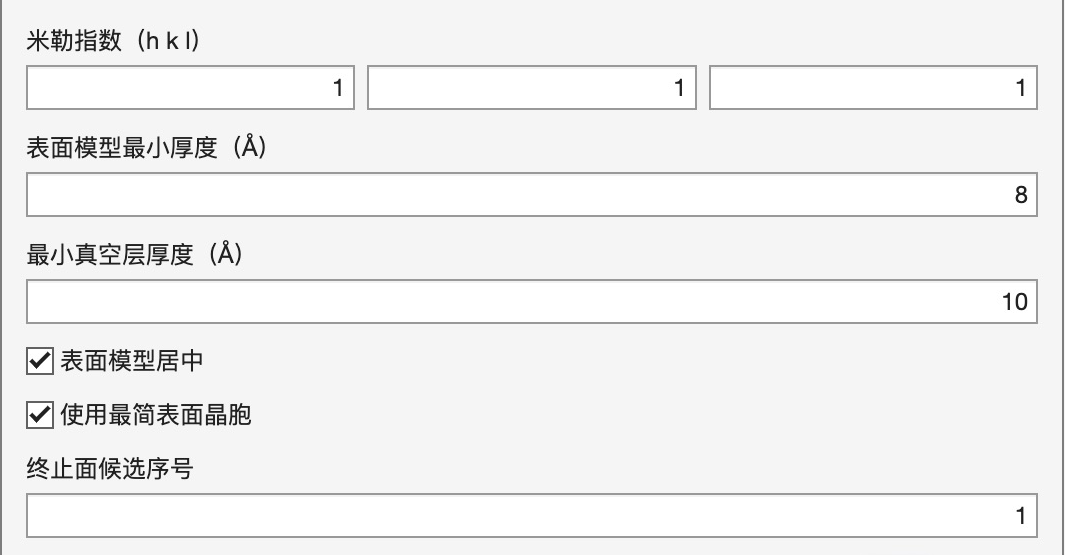
\includegraphics[width=107mm]{publication-assets/crop-e2fa9f70b6bcca245a04.png}
\par\vspace{2mm}
% 同图独立预览提示(975,1460,1520,1495)，545×35；54mm约256ppi，无右侧指针。

\includegraphics[width=54mm]{publication-assets/crop-f2ece60af591133fac37.png}
\caption{Online中导入\file{Pt-fcc.cif}后构建Pt(111)表面的实际参数。米勒指数依次为1、1、1，最小表面厚度为$8\,\text{\AA}$，最小真空层厚度为$10\,\text{\AA}$；启用居中与最简表面晶胞，终止面候选序号为1。下方提示预览已显示，应用后再检查层数与实际间隙。}
\label{fig:pt111-slab-parameters}
\end{figure}
